% Options for packages loaded elsewhere
\PassOptionsToPackage{unicode}{hyperref}
\PassOptionsToPackage{hyphens}{url}
%
\documentclass[
  11pt,
]{article}
\usepackage{amsmath,amssymb}
\usepackage{iftex}
\ifPDFTeX
  \usepackage[T1]{fontenc}
  \usepackage[utf8]{inputenc}
  \usepackage{textcomp} % provide euro and other symbols
\else % if luatex or xetex
  \usepackage{unicode-math} % this also loads fontspec
  \defaultfontfeatures{Scale=MatchLowercase}
  \defaultfontfeatures[\rmfamily]{Ligatures=TeX,Scale=1}
\fi
\usepackage{lmodern}
\ifPDFTeX\else
  % xetex/luatex font selection
\fi
% Use upquote if available, for straight quotes in verbatim environments
\IfFileExists{upquote.sty}{\usepackage{upquote}}{}
\IfFileExists{microtype.sty}{% use microtype if available
  \usepackage[]{microtype}
  \UseMicrotypeSet[protrusion]{basicmath} % disable protrusion for tt fonts
}{}
\makeatletter
\@ifundefined{KOMAClassName}{% if non-KOMA class
  \IfFileExists{parskip.sty}{%
    \usepackage{parskip}
  }{% else
    \setlength{\parindent}{0pt}
    \setlength{\parskip}{6pt plus 2pt minus 1pt}}
}{% if KOMA class
  \KOMAoptions{parskip=half}}
\makeatother
\usepackage{xcolor}
\usepackage[left=1in,right=1in,top=1in,bottom=1in]{geometry}
\usepackage{color}
\usepackage{fancyvrb}
\newcommand{\VerbBar}{|}
\newcommand{\VERB}{\Verb[commandchars=\\\{\}]}
\DefineVerbatimEnvironment{Highlighting}{Verbatim}{commandchars=\\\{\}}
% Add ',fontsize=\small' for more characters per line
\usepackage{framed}
\definecolor{shadecolor}{RGB}{248,248,248}
\newenvironment{Shaded}{\begin{snugshade}}{\end{snugshade}}
\newcommand{\AlertTok}[1]{\textcolor[rgb]{0.94,0.16,0.16}{#1}}
\newcommand{\AnnotationTok}[1]{\textcolor[rgb]{0.56,0.35,0.01}{\textbf{\textit{#1}}}}
\newcommand{\AttributeTok}[1]{\textcolor[rgb]{0.13,0.29,0.53}{#1}}
\newcommand{\BaseNTok}[1]{\textcolor[rgb]{0.00,0.00,0.81}{#1}}
\newcommand{\BuiltInTok}[1]{#1}
\newcommand{\CharTok}[1]{\textcolor[rgb]{0.31,0.60,0.02}{#1}}
\newcommand{\CommentTok}[1]{\textcolor[rgb]{0.56,0.35,0.01}{\textit{#1}}}
\newcommand{\CommentVarTok}[1]{\textcolor[rgb]{0.56,0.35,0.01}{\textbf{\textit{#1}}}}
\newcommand{\ConstantTok}[1]{\textcolor[rgb]{0.56,0.35,0.01}{#1}}
\newcommand{\ControlFlowTok}[1]{\textcolor[rgb]{0.13,0.29,0.53}{\textbf{#1}}}
\newcommand{\DataTypeTok}[1]{\textcolor[rgb]{0.13,0.29,0.53}{#1}}
\newcommand{\DecValTok}[1]{\textcolor[rgb]{0.00,0.00,0.81}{#1}}
\newcommand{\DocumentationTok}[1]{\textcolor[rgb]{0.56,0.35,0.01}{\textbf{\textit{#1}}}}
\newcommand{\ErrorTok}[1]{\textcolor[rgb]{0.64,0.00,0.00}{\textbf{#1}}}
\newcommand{\ExtensionTok}[1]{#1}
\newcommand{\FloatTok}[1]{\textcolor[rgb]{0.00,0.00,0.81}{#1}}
\newcommand{\FunctionTok}[1]{\textcolor[rgb]{0.13,0.29,0.53}{\textbf{#1}}}
\newcommand{\ImportTok}[1]{#1}
\newcommand{\InformationTok}[1]{\textcolor[rgb]{0.56,0.35,0.01}{\textbf{\textit{#1}}}}
\newcommand{\KeywordTok}[1]{\textcolor[rgb]{0.13,0.29,0.53}{\textbf{#1}}}
\newcommand{\NormalTok}[1]{#1}
\newcommand{\OperatorTok}[1]{\textcolor[rgb]{0.81,0.36,0.00}{\textbf{#1}}}
\newcommand{\OtherTok}[1]{\textcolor[rgb]{0.56,0.35,0.01}{#1}}
\newcommand{\PreprocessorTok}[1]{\textcolor[rgb]{0.56,0.35,0.01}{\textit{#1}}}
\newcommand{\RegionMarkerTok}[1]{#1}
\newcommand{\SpecialCharTok}[1]{\textcolor[rgb]{0.81,0.36,0.00}{\textbf{#1}}}
\newcommand{\SpecialStringTok}[1]{\textcolor[rgb]{0.31,0.60,0.02}{#1}}
\newcommand{\StringTok}[1]{\textcolor[rgb]{0.31,0.60,0.02}{#1}}
\newcommand{\VariableTok}[1]{\textcolor[rgb]{0.00,0.00,0.00}{#1}}
\newcommand{\VerbatimStringTok}[1]{\textcolor[rgb]{0.31,0.60,0.02}{#1}}
\newcommand{\WarningTok}[1]{\textcolor[rgb]{0.56,0.35,0.01}{\textbf{\textit{#1}}}}
\usepackage{longtable,booktabs,array}
\usepackage{calc} % for calculating minipage widths
% Correct order of tables after \paragraph or \subparagraph
\usepackage{etoolbox}
\makeatletter
\patchcmd\longtable{\par}{\if@noskipsec\mbox{}\fi\par}{}{}
\makeatother
% Allow footnotes in longtable head/foot
\IfFileExists{footnotehyper.sty}{\usepackage{footnotehyper}}{\usepackage{footnote}}
\makesavenoteenv{longtable}
\usepackage{graphicx}
\makeatletter
\def\maxwidth{\ifdim\Gin@nat@width>\linewidth\linewidth\else\Gin@nat@width\fi}
\def\maxheight{\ifdim\Gin@nat@height>\textheight\textheight\else\Gin@nat@height\fi}
\makeatother
% Scale images if necessary, so that they will not overflow the page
% margins by default, and it is still possible to overwrite the defaults
% using explicit options in \includegraphics[width, height, ...]{}
\setkeys{Gin}{width=\maxwidth,height=\maxheight,keepaspectratio}
% Set default figure placement to htbp
\makeatletter
\def\fps@figure{htbp}
\makeatother
\setlength{\emergencystretch}{3em} % prevent overfull lines
\providecommand{\tightlist}{%
  \setlength{\itemsep}{0pt}\setlength{\parskip}{0pt}}
\setcounter{secnumdepth}{-\maxdimen} % remove section numbering
\usepackage{fvextra}
\DefineVerbatimEnvironment{Highlighting}{Verbatim}{breaklines, breakanywhere, commandchars=\\\{\}}
\ifLuaTeX
  \usepackage{selnolig}  % disable illegal ligatures
\fi
\usepackage{bookmark}
\IfFileExists{xurl.sty}{\usepackage{xurl}}{} % add URL line breaks if available
\urlstyle{same}
\hypersetup{
  pdftitle={POL501 - Problem Set 1},
  pdfauthor={Answers to Questions},
  hidelinks,
  pdfcreator={LaTeX via pandoc}}

\title{POL501 - Problem Set 1}
\author{Answers to Questions}
\date{2024-11-04}

\begin{document}
\maketitle

{
\setcounter{tocdepth}{2}
\tableofcontents
}


\section{Grading Criteria}\label{grading-criteria}

\begin{itemize}
\tightlist
\item
  There will be \textbf{four problem sets} throughout the semester,
  which together account for \textbf{25\% of the final course grade}.
\item
  The total possible score for these problem sets is \textbf{25 out of
  100 points} (with 100 points being the maximum course score).
\item
  This particular problem set has a maximum score of \textbf{7 points}.
\item
  \textbf{Scoring Breakdown}:

  \begin{itemize}
  \tightlist
  \item
    Questions 1 through 5 are worth \textbf{1 point each}.
  \item
    Question 6 is worth \textbf{2 points} (0.25 each letter part).
  \end{itemize}
\item
  \textbf{Grading Guidelines}:

  \begin{itemize}
  \tightlist
  \item
    Full credit will be awarded for answers that closely match the
    provided solutions.
  \item
    Partial credit will be given for incomplete or partially incorrect
    answers/justifications.
  \item
    \textbf{0 points} will be awarded for missing answers, answers with
    no justification, or entirely incorrect responses.
  \end{itemize}
\end{itemize}

\newpage

\section{Answers Problem Set 1.}\label{answers-problem-set-1.}

\subsection{Answer to Question 1}\label{answer-to-question-1}

A study exploring the effects of political corruption on tax compliance
found that in countries with less political corruption, private firms
were less likely to engage in tax fraud.

\textbf{What type of relationship is described in the study?}

\begin{itemize}
\tightlist
\item
  \begin{enumerate}
  \def\labelenumi{(\alph{enumi})}
  \tightlist
  \item
    Positive relationship
  \end{enumerate}
\item
  \begin{enumerate}
  \def\labelenumi{(\alph{enumi})}
  \setcounter{enumi}{1}
  \tightlist
  \item
    Negative relationship
  \end{enumerate}
\item
  \begin{enumerate}
  \def\labelenumi{(\alph{enumi})}
  \setcounter{enumi}{2}
  \tightlist
  \item
    Non-linear relationship
  \end{enumerate}
\item
  \begin{enumerate}
  \def\labelenumi{(\alph{enumi})}
  \setcounter{enumi}{3}
  \tightlist
  \item
    No relationship
  \end{enumerate}
\end{itemize}

\textbf{Answer:} (a) Positive relationship

\textbf{Justification:} The study states that in countries with less
political corruption, private firms are less likely to engage in tax
fraud. This indicates that as corruption decreases, tax fraud decreases,
showing a positive relationship because both variables change in the
same direction.

However, note that the relationship described in the study depends on
how we frame the variables. If we measure tax fraud (or non-compliance)
against political corruption, a \emph{positive relationship} means that
as corruption decreases, tax fraud also decreases. However, if we
instead focus on \emph{tax compliance} as the variable, the relationship
becomes \emph{negative}: as corruption decreases, tax compliance
increases. This reversal occurs because tax compliance and tax fraud are
opposites. It's crucial to clearly define which variables we are
measuring and their directions to avoid confusion when interpreting
relationships between them. Clear identification ensures accurate
understanding of the study's findings.

\hrule

\subsection{Answer to Question 2}\label{answer-to-question-2}

A study found that as the number of community events increases from a
few to a moderate number, community cohesion improves. However, when the
number of events increases from moderate to high, community cohesion
decreases.

\textbf{What kind of association is this?}

\begin{itemize}
\tightlist
\item
  \begin{enumerate}
  \def\labelenumi{(\alph{enumi})}
  \tightlist
  \item
    Positive association
  \end{enumerate}
\item
  \begin{enumerate}
  \def\labelenumi{(\alph{enumi})}
  \setcounter{enumi}{1}
  \tightlist
  \item
    Negative association
  \end{enumerate}
\item
  \begin{enumerate}
  \def\labelenumi{(\alph{enumi})}
  \setcounter{enumi}{2}
  \tightlist
  \item
    Non-linear association
  \end{enumerate}
\item
  \begin{enumerate}
  \def\labelenumi{(\alph{enumi})}
  \setcounter{enumi}{3}
  \tightlist
  \item
    The variables are independent of each other
  \end{enumerate}
\end{itemize}

\textbf{Answer:} (c) Non-linear association

\textbf{Justification:} The study found that community cohesion improves
with an increase in community events up to a moderate number, but then
decreases as the number of events becomes high. This indicates a
non-linear association, where the relationship between community events
and cohesion changes direction at different levels.

\hrule

\subsection{Answer to Question 3}\label{answer-to-question-3}

A study of one recent primary for the Republican party revealed the
following data. Researchers were surprised to observe the results.

\begin{longtable}[]{@{}lll@{}}
\toprule\noalign{}
Candidate Names & Total Votes Won & Campaign Spending (\$) \\
\midrule\noalign{}
\endhead
\bottomrule\noalign{}
\endlastfoot
Candidate A & 10,000 & 500,000 \\
Candidate B & 15,000 & 300,000 \\
Candidate C & 8,000 & 700,000 \\
Candidate D & 12,000 & 400,000 \\
\end{longtable}

\textbf{According to this data table, what kind of association is found
between ``spending'' and ``votes''?}

\begin{itemize}
\tightlist
\item
  \begin{enumerate}
  \def\labelenumi{(\alph{enumi})}
  \tightlist
  \item
    Positive association
  \end{enumerate}
\item
  \begin{enumerate}
  \def\labelenumi{(\alph{enumi})}
  \setcounter{enumi}{1}
  \tightlist
  \item
    Negative association
  \end{enumerate}
\item
  \begin{enumerate}
  \def\labelenumi{(\alph{enumi})}
  \setcounter{enumi}{2}
  \tightlist
  \item
    Non-linear association
  \end{enumerate}
\item
  \begin{enumerate}
  \def\labelenumi{(\alph{enumi})}
  \setcounter{enumi}{3}
  \tightlist
  \item
    The variables are independent of each other
  \end{enumerate}
\end{itemize}

\textbf{Answer:} (b) Negative association

\textbf{Justification:} By examining the data table and sorting the
candidates by spending shows that higher spending generally corresponds
to fewer votes:

\begin{itemize}
\tightlist
\item
  Candidate B: \$300,000, 15,000 votes
\item
  Candidate D: \$400,000, 12,000 votes
\item
  Candidate A: \$500,000, 10,000 votes
\item
  Candidate C: \$700,000, 8,000 votes
\end{itemize}

This pattern suggests a negative association where higher spending is
associated with fewer votes. Therefore, there is a negative relationship
between the two variables.

We can confirm this by also plotting the two variables in a scatter
plot.

\begin{Shaded}
\begin{Highlighting}[]
\CommentTok{\# Create the dataframe}
\NormalTok{candidate\_data }\OtherTok{\textless{}{-}} \FunctionTok{data.frame}\NormalTok{(}
  \AttributeTok{Candidate\_Names =} \FunctionTok{c}\NormalTok{(}\StringTok{"Candidate A"}\NormalTok{, }\StringTok{"Candidate B"}\NormalTok{, }\StringTok{"Candidate C"}\NormalTok{, }
                      \StringTok{"Candidate D"}\NormalTok{),}
  \AttributeTok{Total\_Votes\_Won =} \FunctionTok{c}\NormalTok{(}\DecValTok{10000}\NormalTok{, }\DecValTok{15000}\NormalTok{, }\DecValTok{8000}\NormalTok{, }\DecValTok{12000}\NormalTok{),}
  \AttributeTok{Campaign\_Spending =} \FunctionTok{c}\NormalTok{(}\DecValTok{500000}\NormalTok{, }\DecValTok{300000}\NormalTok{, }\DecValTok{700000}\NormalTok{, }\DecValTok{400000}\NormalTok{)}
\NormalTok{)}

\CommentTok{\# View the dataframe}
\FunctionTok{print}\NormalTok{(candidate\_data)}
\end{Highlighting}
\end{Shaded}

\begin{verbatim}
##   Candidate_Names Total_Votes_Won Campaign_Spending
## 1     Candidate A           10000             5e+05
## 2     Candidate B           15000             3e+05
## 3     Candidate C            8000             7e+05
## 4     Candidate D           12000             4e+05
\end{verbatim}

\begin{Shaded}
\begin{Highlighting}[]
\CommentTok{\# Set plot dimensions (width, height) in inches}
\FunctionTok{par}\NormalTok{(}\AttributeTok{pin =} \FunctionTok{c}\NormalTok{(}\DecValTok{4}\NormalTok{, }\FloatTok{2.5}\NormalTok{))  }\CommentTok{\# Example: 4 inches wide, 2.5 inches tall}

\CommentTok{\# Plot the relationship between Total Votes and Campaign Spending}
\FunctionTok{plot}\NormalTok{(}\AttributeTok{x=}\NormalTok{candidate\_data}\SpecialCharTok{$}\NormalTok{Campaign\_Spending,}
  \AttributeTok{y=}\NormalTok{candidate\_data}\SpecialCharTok{$}\NormalTok{Total\_Votes\_Won, }
  \AttributeTok{xlab =} \StringTok{"Campaign Spending ($)"}\NormalTok{, }
  \AttributeTok{ylab =} \StringTok{"Total Votes Won"}\NormalTok{,}
  \AttributeTok{main =} \StringTok{"Relationship between Campaign Spending and Total Votes Won"}\NormalTok{,}
  \AttributeTok{pch =} \DecValTok{19}\NormalTok{, }\AttributeTok{col =} \StringTok{"blue"}
\NormalTok{)}
\end{Highlighting}
\end{Shaded}

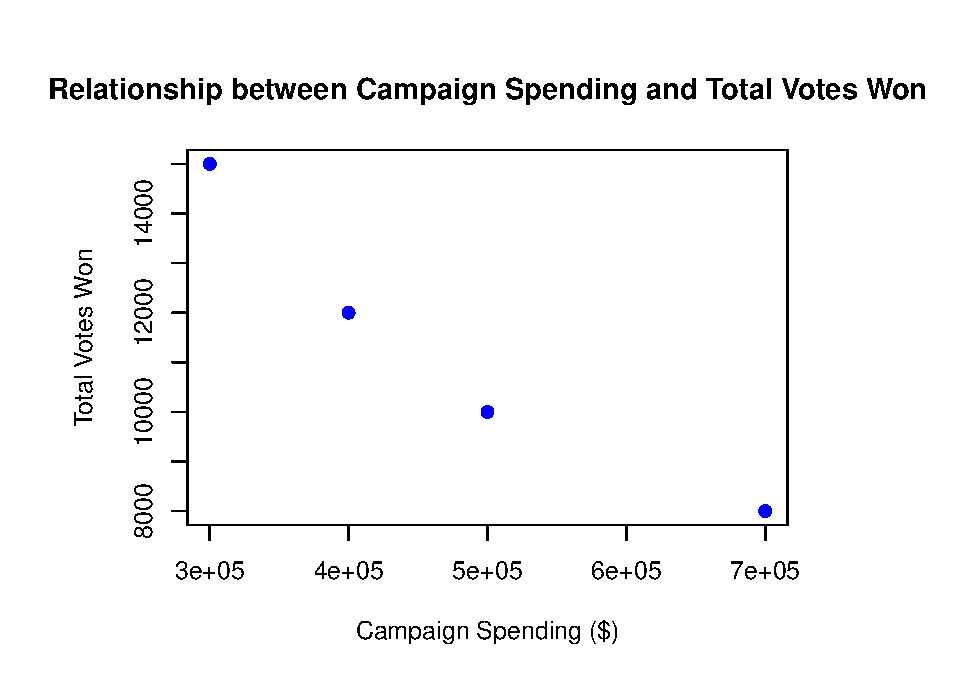
\includegraphics{Problem-Sets/Answers-Files/Answers-PS1/unnamed-chunk-1-1.pdf}

\hrule

\subsection{Answer to Question 4}\label{answer-to-question-4}

Consider the level of satisfaction with local government services as
expressed through a survey using ratings: very unsatisfied, unsatisfied,
neutral, satisfied, very satisfied. This question assesses the perceived
effectiveness of services such as public transportation, parks, and
emergency responses.

\textbf{Which kind of variable type is this?}

\begin{itemize}
\tightlist
\item
  \begin{enumerate}
  \def\labelenumi{(\alph{enumi})}
  \tightlist
  \item
    Regular Categorical (Nominal)
  \end{enumerate}
\item
  \begin{enumerate}
  \def\labelenumi{(\alph{enumi})}
  \setcounter{enumi}{1}
  \tightlist
  \item
    Ordinal Categorical (Ordinal)
  \end{enumerate}
\item
  \begin{enumerate}
  \def\labelenumi{(\alph{enumi})}
  \setcounter{enumi}{2}
  \tightlist
  \item
    Numerical (Discrete)
  \end{enumerate}
\item
  \begin{enumerate}
  \def\labelenumi{(\alph{enumi})}
  \setcounter{enumi}{3}
  \tightlist
  \item
    Numerical (Continuous)
  \end{enumerate}
\end{itemize}

\textbf{Answer:} (b) Ordinal Categorical (Ordinal)

\textbf{Justification:} The levels of satisfaction (very unsatisfied,
unsatisfied, neutral, satisfied, very satisfied) are ordered categories.
This makes the variable ordinal since it has a meaningful order but the
intervals between levels are not necessarily equal.

\hrule

\subsection{Answer to Question 5}\label{answer-to-question-5}

In a psychological study examining stress triggers, participants were
categorized by their primary work environment settings, such as
`open-plan offices', `private offices', and `remote work from home'.
Researchers sought to determine if these settings influenced reported
stress levels during work hours.

\textbf{Which is the explanatory variable and which is the response?}

\begin{itemize}
\tightlist
\item
  \begin{enumerate}
  \def\labelenumi{(\alph{enumi})}
  \tightlist
  \item
    Work environment setting is the response, and stress level is the
    explanatory variable.
  \end{enumerate}
\item
  \begin{enumerate}
  \def\labelenumi{(\alph{enumi})}
  \setcounter{enumi}{1}
  \tightlist
  \item
    Stress level is the response, and work environment setting is the
    explanatory variable.
  \end{enumerate}
\end{itemize}

\textbf{Answer:} (b) Stress level is the response, and work environment
setting is the explanatory variable.

\textbf{Justification:} The study examines how different work
environment settings (open-plan offices, private offices, remote work
from home) influence the reported stress levels of participants.
Therefore, the work environment setting is the explanatory variable
(independent variable), and the stress level is the response variable
(dependent variable).

\hrule

\subsection{Answer to Question 6}\label{answer-to-question-6}

\subsubsection{Part (a)}\label{part-a}

\textbf{Mean, Median, and Standard Deviation}

We will calculate the mean, median, and standard deviation for both the
number of social activities per month and the social trust levels across
the neighborhoods.

The algebraic formulas are: \[
   \text{Mean} (\mu) = \frac{1}{N} \sum_{i=1}^{N} x_i
   \] \[
   \text{Median: Arrange the data in ascending order and find the middle value.}
   \] \[
   \text{Standard Deviation} (\sigma) = \sqrt{\frac{1}{N} \sum_{i=1}^{N} (x_i - \mu)^2}
   \]

We can create a dataframe and use dyplyr or base R to do the
calculations.

\begin{Shaded}
\begin{Highlighting}[]
\CommentTok{\# Create the data vectors}
\NormalTok{neighborhood\_id }\OtherTok{\textless{}{-}} \FunctionTok{c}\NormalTok{(}\StringTok{"N1"}\NormalTok{, }\StringTok{"N2"}\NormalTok{, }\StringTok{"N3"}\NormalTok{, }\StringTok{"N4"}\NormalTok{, }\StringTok{"N5"}\NormalTok{, }\StringTok{"N6"}\NormalTok{, }\StringTok{"N7"}\NormalTok{, }\StringTok{"N8"}\NormalTok{, }\StringTok{"N9"}\NormalTok{, }\StringTok{"N10"}\NormalTok{,}
    \StringTok{"N11"}\NormalTok{)}
\NormalTok{number\_of\_social\_activities }\OtherTok{\textless{}{-}} \FunctionTok{c}\NormalTok{(}\DecValTok{1}\NormalTok{, }\FloatTok{2.9}\NormalTok{, }\FloatTok{4.8}\NormalTok{, }\FloatTok{6.7}\NormalTok{, }\FloatTok{8.6}\NormalTok{, }\FloatTok{10.5}\NormalTok{, }\FloatTok{12.4}\NormalTok{, }\FloatTok{14.3}\NormalTok{, }\FloatTok{16.2}\NormalTok{, }\FloatTok{18.1}\NormalTok{,}
    \DecValTok{20}\NormalTok{)}
\NormalTok{social\_trust\_index }\OtherTok{\textless{}{-}} \FunctionTok{c}\NormalTok{(}\FloatTok{21.48}\NormalTok{, }\FloatTok{48.9}\NormalTok{, }\FloatTok{76.2}\NormalTok{, }\FloatTok{96.73}\NormalTok{, }\FloatTok{96.87}\NormalTok{, }\FloatTok{98.58}\NormalTok{, }\FloatTok{102.14}\NormalTok{, }\FloatTok{85.35}\NormalTok{, }\FloatTok{59.21}\NormalTok{,}
    \FloatTok{37.1}\NormalTok{, }\FloatTok{1.2}\NormalTok{)}

\CommentTok{\# Create the dataframe}
\NormalTok{df }\OtherTok{\textless{}{-}} \FunctionTok{data.frame}\NormalTok{(neighborhood\_id, number\_of\_social\_activities, social\_trust\_index)}

\CommentTok{\# View the dataframe}
\FunctionTok{print}\NormalTok{(df)}
\end{Highlighting}
\end{Shaded}

\begin{verbatim}
##    neighborhood_id number_of_social_activities social_trust_index
## 1               N1                         1.0              21.48
## 2               N2                         2.9              48.90
## 3               N3                         4.8              76.20
## 4               N4                         6.7              96.73
## 5               N5                         8.6              96.87
## 6               N6                        10.5              98.58
## 7               N7                        12.4             102.14
## 8               N8                        14.3              85.35
## 9               N9                        16.2              59.21
## 10             N10                        18.1              37.10
## 11             N11                        20.0               1.20
\end{verbatim}

\begin{Shaded}
\begin{Highlighting}[]
\CommentTok{\# Using Base R:}

\CommentTok{\# Calculate mean, median, and standard deviation for}
\CommentTok{\# number\_of\_social\_activities}
\NormalTok{mean\_activities }\OtherTok{\textless{}{-}} \FunctionTok{mean}\NormalTok{(df}\SpecialCharTok{$}\NormalTok{number\_of\_social\_activities)}
\NormalTok{median\_activities }\OtherTok{\textless{}{-}} \FunctionTok{median}\NormalTok{(df}\SpecialCharTok{$}\NormalTok{number\_of\_social\_activities)}
\NormalTok{sd\_activities }\OtherTok{\textless{}{-}} \FunctionTok{sd}\NormalTok{(df}\SpecialCharTok{$}\NormalTok{number\_of\_social\_activities)}

\CommentTok{\# Calculate mean, median, and standard deviation for social\_trust\_index}
\NormalTok{mean\_trust }\OtherTok{\textless{}{-}} \FunctionTok{mean}\NormalTok{(df}\SpecialCharTok{$}\NormalTok{social\_trust\_index)}
\NormalTok{median\_trust }\OtherTok{\textless{}{-}} \FunctionTok{median}\NormalTok{(df}\SpecialCharTok{$}\NormalTok{social\_trust\_index)}
\NormalTok{sd\_trust }\OtherTok{\textless{}{-}} \FunctionTok{sd}\NormalTok{(df}\SpecialCharTok{$}\NormalTok{social\_trust\_index)}

\CommentTok{\# Print the results}
\FunctionTok{cat}\NormalTok{(}\StringTok{"Base R Summary Statistics:}\SpecialCharTok{\textbackslash{}n}\StringTok{"}\NormalTok{)}
\end{Highlighting}
\end{Shaded}

\begin{verbatim}
## Base R Summary Statistics:
\end{verbatim}

\begin{Shaded}
\begin{Highlighting}[]
\FunctionTok{cat}\NormalTok{(}\StringTok{"Number of Social Activities {-} Mean:"}\NormalTok{, mean\_activities, }\StringTok{", Median:"}\NormalTok{, median\_activities,}
    \StringTok{", SD:"}\NormalTok{, sd\_activities, }\StringTok{"}\SpecialCharTok{\textbackslash{}n}\StringTok{"}\NormalTok{)}
\end{Highlighting}
\end{Shaded}

\begin{verbatim}
## Number of Social Activities - Mean: 10.5 , Median: 10.5 , SD: 6.301587
\end{verbatim}

\begin{Shaded}
\begin{Highlighting}[]
\FunctionTok{cat}\NormalTok{(}\StringTok{"Social Trust Index {-} Mean:"}\NormalTok{, mean\_trust, }\StringTok{", Median:"}\NormalTok{, median\_trust, }\StringTok{", SD:"}\NormalTok{,}
\NormalTok{    sd\_trust, }\StringTok{"}\SpecialCharTok{\textbackslash{}n}\StringTok{"}\NormalTok{)}
\end{Highlighting}
\end{Shaded}

\begin{verbatim}
## Social Trust Index - Mean: 65.79636 , Median: 76.2 , SD: 34.78167
\end{verbatim}

Alternatively we can use the package \texttt{dyplyr} and get the output
in a dataframe. Importantly, the code here allows to get the summary
statistics for each variable organized by rows. This is format is easy
to read and good for reports.

\begin{Shaded}
\begin{Highlighting}[]
\CommentTok{\# Install dplyr if it\textquotesingle{}s not already installed}
\CommentTok{\# install.packages("dplyr")}

\CommentTok{\# Load dplyr}
\FunctionTok{library}\NormalTok{(dplyr)}


\CommentTok{\# Compute summary statistics for \textquotesingle{}number\_of\_social\_activities\textquotesingle{}}
\NormalTok{stats\_activities }\OtherTok{\textless{}{-}}\NormalTok{ df }\SpecialCharTok{\%\textgreater{}\%}
  \FunctionTok{summarise}\NormalTok{(}
    \AttributeTok{Variable =} \StringTok{"Number of Social Activities"}\NormalTok{,}
    \AttributeTok{Mean =} \FunctionTok{mean}\NormalTok{(number\_of\_social\_activities),}
    \AttributeTok{Median =} \FunctionTok{median}\NormalTok{(number\_of\_social\_activities),}
    \AttributeTok{SD =} \FunctionTok{sd}\NormalTok{(number\_of\_social\_activities)}
\NormalTok{  )}

\CommentTok{\# Compute summary statistics for \textquotesingle{}social\_trust\_index\textquotesingle{}}
\NormalTok{stats\_trust }\OtherTok{\textless{}{-}}\NormalTok{ df }\SpecialCharTok{\%\textgreater{}\%}
  \FunctionTok{summarise}\NormalTok{(}
    \AttributeTok{Variable =} \StringTok{"Social Trust Index"}\NormalTok{,}
    \AttributeTok{Mean =} \FunctionTok{mean}\NormalTok{(social\_trust\_index),}
    \AttributeTok{Median =} \FunctionTok{median}\NormalTok{(social\_trust\_index),}
    \AttributeTok{SD =} \FunctionTok{sd}\NormalTok{(social\_trust\_index)}
\NormalTok{  )}

\CommentTok{\# Combine the two data frames}
\NormalTok{summary\_stats\_dplyr }\OtherTok{\textless{}{-}} \FunctionTok{bind\_rows}\NormalTok{(stats\_activities, stats\_trust)}

\CommentTok{\# View the summary statistics}
\FunctionTok{print}\NormalTok{(summary\_stats\_dplyr)}
\end{Highlighting}
\end{Shaded}

\begin{verbatim}
##                      Variable     Mean Median        SD
## 1 Number of Social Activities 10.50000   10.5  6.301587
## 2          Social Trust Index 65.79636   76.2 34.781671
\end{verbatim}

Final Results:

\begin{itemize}
\tightlist
\item
  Number of Social Activities (per month):

  \begin{itemize}
  \tightlist
  \item
    Mean: 10.5
  \item
    Median: 10.5
  \item
    Standard Deviation: 6.3
  \end{itemize}
\item
  Social Trust Level (out of 100):

  \begin{itemize}
  \tightlist
  \item
    Mean: 65.79
  \item
    Median: 76.2
  \item
    Standard Deviation: 34.78
  \end{itemize}
\end{itemize}

\textbf{Interpretation:}

\begin{itemize}
\tightlist
\item
  Number of Social Activities:

  \begin{itemize}
  \tightlist
  \item
    The mean and median being equal (10.5) indicates a symmetric
    distribution.
  \item
    The standard deviation of 6.01 suggests moderate variability around
    the mean.
  \end{itemize}
\item
  Social Trust Level:

  \begin{itemize}
  \tightlist
  \item
    The mean (65.79) and median (76.2) indicate a skewed distribution,
    likely left-skewed because the mean is less than the median.
  \item
    The high standard deviation (34.78) indicates high variability in
    social trust levels among the neighborhoods.
  \end{itemize}
\end{itemize}

\textbf{Note:} \texttt{bind\_rows()} in R combines multiple data frames
or data-like objects (such as tibbles) by stacking them vertically,
i.e., adding rows from one below the other. It automatically matches
columns by name, filling in missing values with \texttt{NA} if a column
is not present in all data frames.

\subsubsection{Part (b)}\label{part-b}

\textbf{Histogram}

We will create a histogram for both the number of social activities per
month and the social trust levels with five bins of equal size. We will
divide the data range into five equal-sized bins for both variables. We
count how many observations fall unto each bin. We use these frequency
counts as the values for the y-axis.

\begin{Shaded}
\begin{Highlighting}[]
\CommentTok{\# Install ggplot2 if not already installed install.packages(\textquotesingle{}ggplot2\textquotesingle{})}

\CommentTok{\# Load ggplot2}
\FunctionTok{library}\NormalTok{(ggplot2)}

\CommentTok{\# Manually specify bin boundaries for Number of Social Activities}
\NormalTok{min\_activities }\OtherTok{\textless{}{-}} \DecValTok{0}  \CommentTok{\# Minimum theoretical value}
\NormalTok{max\_activities }\OtherTok{\textless{}{-}} \FunctionTok{max}\NormalTok{(df}\SpecialCharTok{$}\NormalTok{number\_of\_social\_activities)  }\CommentTok{\# Max value from the data}
\NormalTok{bin\_breaks\_activities }\OtherTok{\textless{}{-}} \FunctionTok{seq}\NormalTok{(min\_activities, max\_activities, }\AttributeTok{length.out =} \DecValTok{6}\NormalTok{)  }\CommentTok{\# 5 bins require 6 boundaries}

\CommentTok{\# Manually specify bin boundaries for Social Trust Index}
\NormalTok{min\_trust }\OtherTok{\textless{}{-}} \DecValTok{0}  \CommentTok{\# Minimum theoretical value}
\NormalTok{max\_trust }\OtherTok{\textless{}{-}} \FunctionTok{max}\NormalTok{(df}\SpecialCharTok{$}\NormalTok{social\_trust\_index)  }\CommentTok{\# Maximum value from the data}
\NormalTok{bin\_breaks\_trust }\OtherTok{\textless{}{-}} \FunctionTok{seq}\NormalTok{(min\_trust, max\_trust, }\AttributeTok{length.out =} \DecValTok{6}\NormalTok{)  }\CommentTok{\# 5 bins require 6 boundaries}
\end{Highlighting}
\end{Shaded}

\begin{Shaded}
\begin{Highlighting}[]
\CommentTok{\# Histogram for Number of Social Activities with manually specified bins}
\FunctionTok{ggplot}\NormalTok{(df, }\FunctionTok{aes}\NormalTok{(}\AttributeTok{x =}\NormalTok{ number\_of\_social\_activities)) }\SpecialCharTok{+} \FunctionTok{geom\_histogram}\NormalTok{(}\AttributeTok{breaks =}\NormalTok{ bin\_breaks\_activities,}
    \AttributeTok{fill =} \StringTok{"lightblue"}\NormalTok{, }\AttributeTok{color =} \StringTok{"black"}\NormalTok{) }\SpecialCharTok{+} \FunctionTok{labs}\NormalTok{(}\AttributeTok{title =} \StringTok{"Histogram of Number of Social Activities"}\NormalTok{,}
    \AttributeTok{x =} \StringTok{"Number of Social Activities"}\NormalTok{, }\AttributeTok{y =} \StringTok{"Frequency"}\NormalTok{) }\SpecialCharTok{+} \FunctionTok{theme\_minimal}\NormalTok{()}
\end{Highlighting}
\end{Shaded}

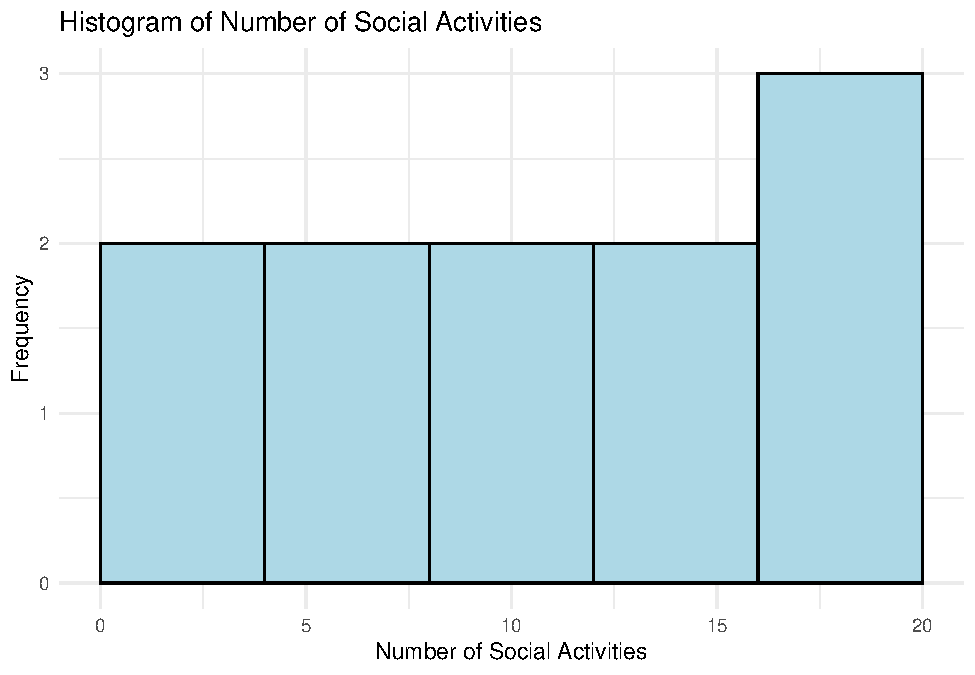
\includegraphics{Problem-Sets/Answers-Files/Answers-PS1/unnamed-chunk-5-1.pdf}

\begin{Shaded}
\begin{Highlighting}[]
\CommentTok{\# Histogram for Social Trust Index with manually specified bins}
\FunctionTok{ggplot}\NormalTok{(df, }\FunctionTok{aes}\NormalTok{(}\AttributeTok{x =}\NormalTok{ social\_trust\_index)) }\SpecialCharTok{+} \FunctionTok{geom\_histogram}\NormalTok{(}\AttributeTok{breaks =}\NormalTok{ bin\_breaks\_trust,}
    \AttributeTok{fill =} \StringTok{"lightgreen"}\NormalTok{, }\AttributeTok{color =} \StringTok{"black"}\NormalTok{) }\SpecialCharTok{+} \FunctionTok{labs}\NormalTok{(}\AttributeTok{title =} \StringTok{"Histogram of Social Trust Index"}\NormalTok{,}
    \AttributeTok{x =} \StringTok{"Social Trust Index"}\NormalTok{, }\AttributeTok{y =} \StringTok{"Frequency"}\NormalTok{) }\SpecialCharTok{+} \FunctionTok{theme\_minimal}\NormalTok{()}
\end{Highlighting}
\end{Shaded}

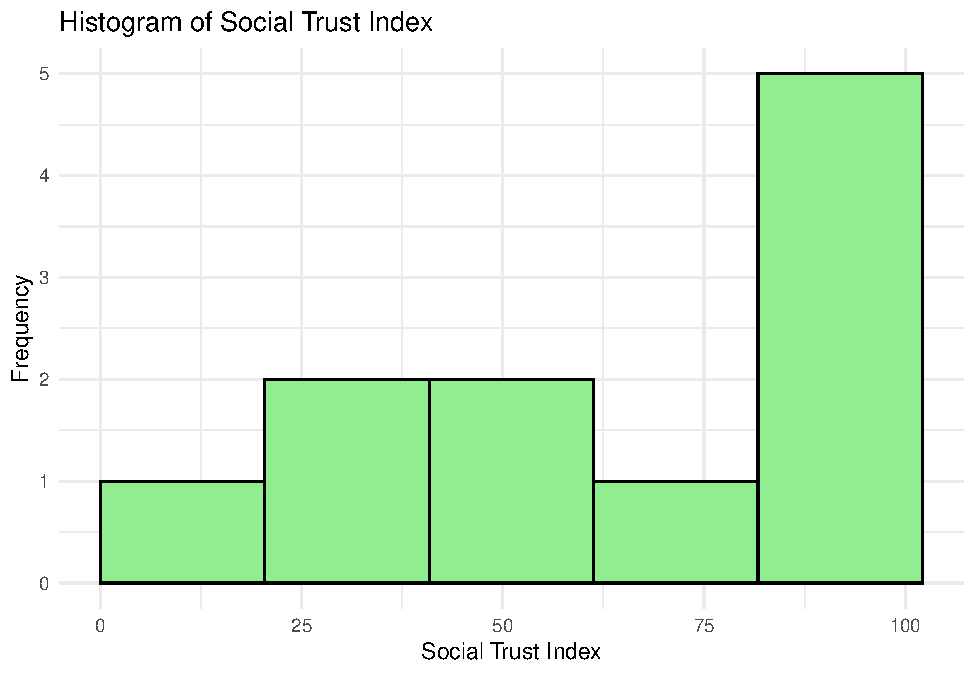
\includegraphics{Problem-Sets/Answers-Files/Answers-PS1/unnamed-chunk-6-1.pdf}

\textbf{Final Results:}

\begin{itemize}
\tightlist
\item
  Number of Social Activities:

  \begin{itemize}
  \tightlist
  \item
    The histogram shows a roughly symmetric distribution.
  \item
    The data is concentrated around the mean.
  \item
    The distribution is unimodal.
  \end{itemize}
\item
  Social Trust Levels:

  \begin{itemize}
  \tightlist
  \item
    The histogram shows a skewed distribution, likely left-skewed.
  \item
    There is a high concentration of data points at higher trust levels,
    with a tail extending towards lower trust levels.
  \item
    The distribution is unimodal.
  \end{itemize}
\end{itemize}

\subsubsection{Part (c)}\label{part-c}

\textbf{Scatter Plot}

\begin{itemize}
\tightlist
\item
  We will create a scatter plot between the number of social activities
  and social trust levels.
\item
  We will plot each pair \((x_i, y_i)\) where \(x_i\) is the number of
  social activities and \(y_i\) is the social trust level.
\end{itemize}

\begin{Shaded}
\begin{Highlighting}[]
\CommentTok{\# Note: Because we already loaded ggplot in a previous code chunk, we dont need}
\CommentTok{\# to do it again.}

\CommentTok{\# Scatter plot using ggplot2}
\FunctionTok{ggplot}\NormalTok{(df, }\FunctionTok{aes}\NormalTok{(}\AttributeTok{x =}\NormalTok{ number\_of\_social\_activities, }\AttributeTok{y =}\NormalTok{ social\_trust\_index)) }\SpecialCharTok{+} \FunctionTok{geom\_point}\NormalTok{(}\AttributeTok{color =} \StringTok{"blue"}\NormalTok{,}
    \AttributeTok{size =} \DecValTok{3}\NormalTok{) }\SpecialCharTok{+} \FunctionTok{labs}\NormalTok{(}\AttributeTok{title =} \StringTok{"Scatter Plot of Social Activities vs Social Trust"}\NormalTok{,}
    \AttributeTok{x =} \StringTok{"Number of Social Activities"}\NormalTok{, }\AttributeTok{y =} \StringTok{"Social Trust Index"}\NormalTok{) }\SpecialCharTok{+} \FunctionTok{theme\_minimal}\NormalTok{()}
\end{Highlighting}
\end{Shaded}

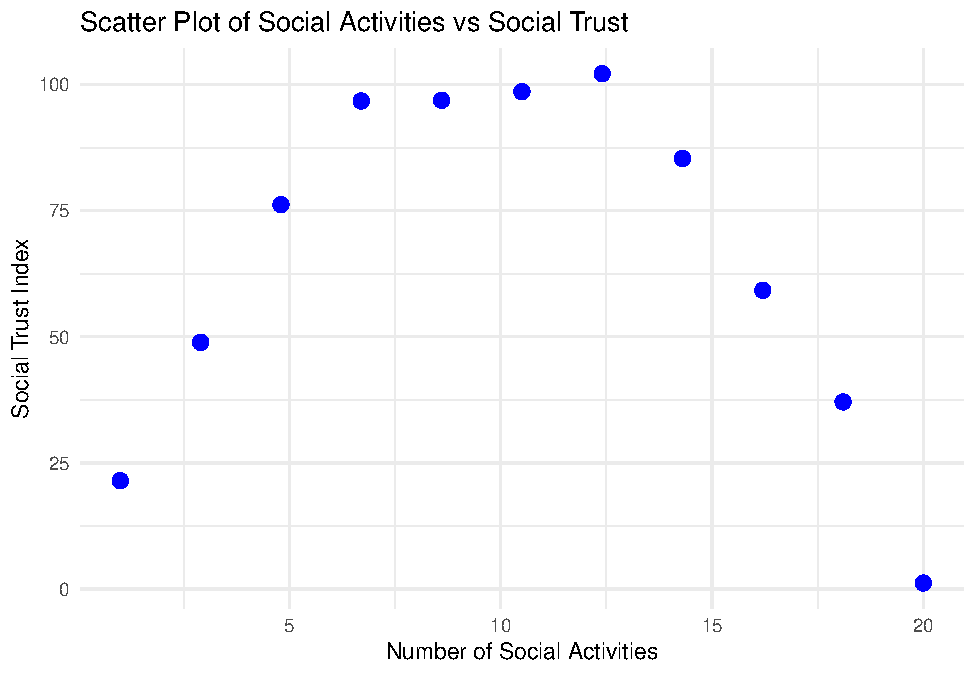
\includegraphics{Problem-Sets/Answers-Files/Answers-PS1/unnamed-chunk-7-1.pdf}

\textbf{Interpretation:}

\begin{itemize}
\tightlist
\item
  The scatter plot shows a clear pattern where the social trust level
  increases with the number of social activities up to a point, and then
  it appears to decrease.
\item
  This suggests a non-linear relationship between the number of social
  activities and social trust levels.
\end{itemize}

\subsubsection{Part (d)}\label{part-d}

\textbf{Hypothesis:} There is a non-linear relationship between the
number of social activities and social trust levels. Initially, more
social activities correlate with higher social trust, but after reaching
a peak, further increases in social activities are associated with a
decrease in social trust.

\begin{itemize}
\tightlist
\item
  Initially, increased social activities may help build community bonds
  and trust as more interactions occur.
\item
  However, beyond a certain threshold, too many social activities could
  become overwhelming, leading to stress or a feeling of obligatory
  participation, which might reduce overall trust levels.
\item
  This indicates the importance of balancing the number of social
  activities to maintain optimal levels of social trust within
  communities.
\end{itemize}

\end{document}
